\documentclass{beamer}

% packages
\usepackage[utf8]{inputenc}
\usepackage{graphicx}
\usepackage{indentfirst}
\usepackage{amsmath}
\usepackage{geometry}
\usepackage{amsthm}
\usepackage{amssymb}
\usepackage{graphicx}
\usepackage{float}
\usepackage{setspace}
\usepackage{booktabs}
\usepackage{tabularx,colortbl}
%\usepackage[colorlinks=true,linkcolor=black]{hyperref}
\usepackage{fancyhdr}
%\pagestyle{fancy}
\usepackage{textcomp}
\usepackage{setspace}
\usepackage{lineno}


% theme
\usetheme{Ilmenau}
\usecolortheme{beaver}


\title{Reconstruct Population Dynamics of White-tailed Deer in Suburb Chicago under Intensive Culling}
\author{Yunyi SHEN}
\institute{UW Madison\\ Department of Forest and Wildlife Ecology}
\date{\today}

\begin{document}
\frame{\titlepage}
\frame{\tableofcontents}

\section{Introduction}
\begin{frame}{Introduction}
	\begin{itemize}
		\item Suburb Deer Problem
		\item Intensive Culling
	\end{itemize}
\end{frame}

\subsection{Suburb Deer Problem}

\begin{frame}{Deer are There: Fawn Found in Chicago}
	\begin{figure}[ht]
		\centering
		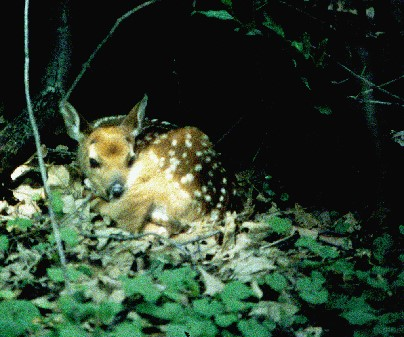
\includegraphics[scale=.5]{fig/Chicago_deer/fawn.jpg}
		%\caption{Wilson}
		\label{fawn}
	\end{figure}
\end{frame}

\begin{frame}{Overabundant Deer is a Problem: Collision}
	\begin{figure}[ht]
		\centering
		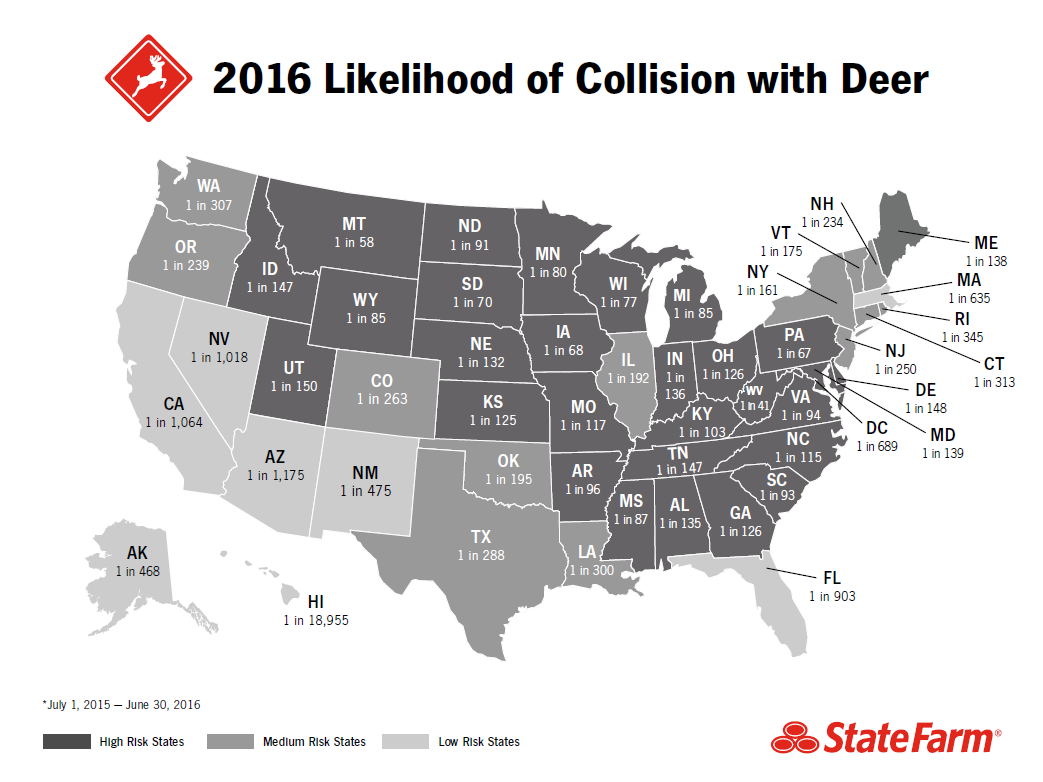
\includegraphics[scale=.23]{fig/Chicago_deer/1920_deermap.png}
		%\caption{Wilson}
		\label{deermap}
	\end{figure}
\end{frame}

\begin{frame}{Overabundant Deer is a Problem: CWD}
	\begin{figure}[ht]
		\centering
		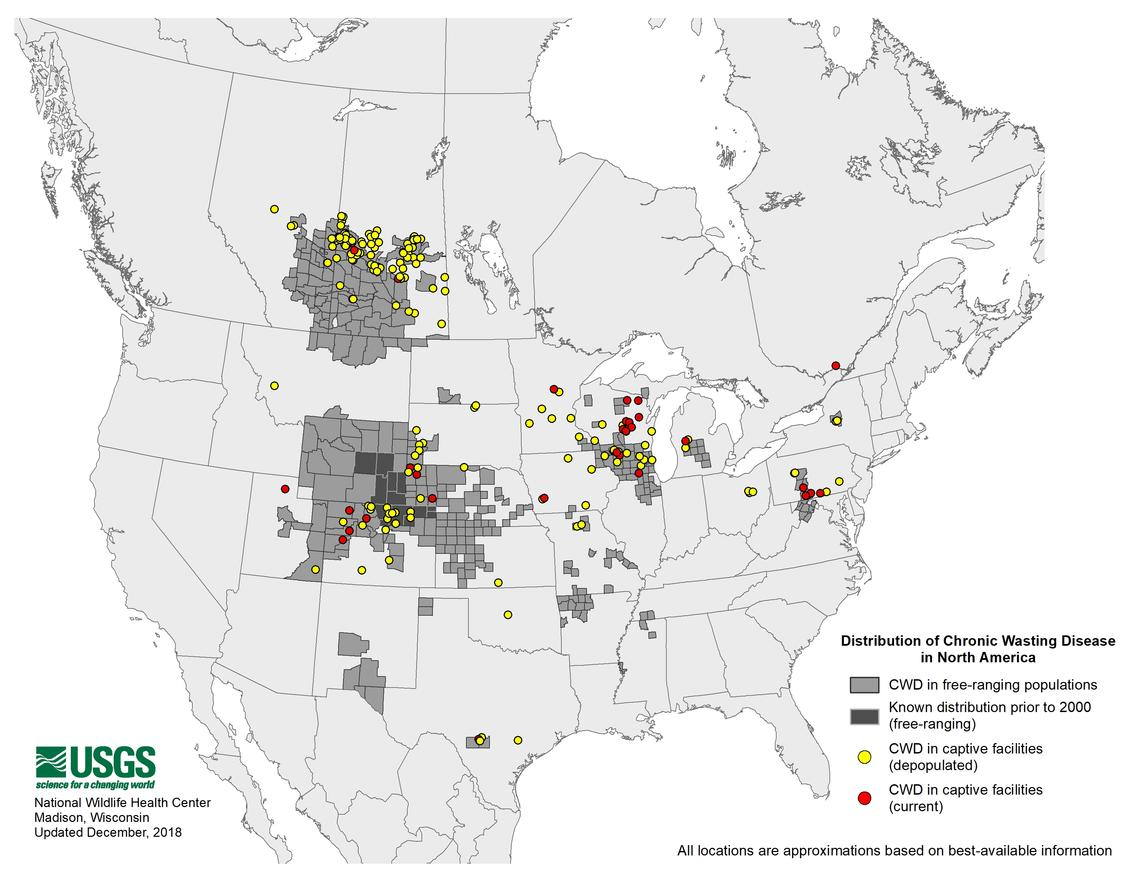
\includegraphics[scale=0.8]{fig/Chicago_deer/CWD.jpg}
		%\caption{Wilson}
		\label{cwd}
	\end{figure}
\end{frame}



\subsection{Intensive Culling}

\begin{frame}{How do People do in Chicago}
	\begin{itemize}
		\item Intensive Culling!
	\end{itemize}
	\begin{figure}[ht]
		\centering
		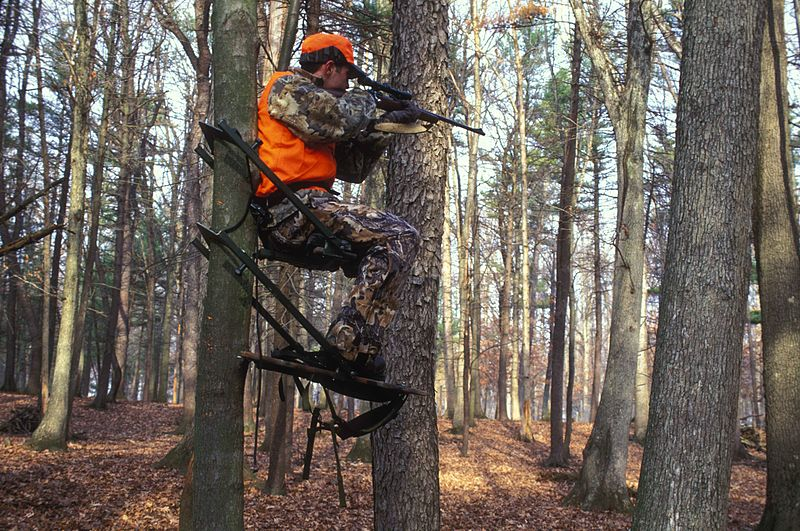
\includegraphics[scale=8]{fig/Chicago_deer/hunting.jpg}
		%\caption{Wilson}
		\label{sample_graph}
	\end{figure}
\end{frame}

\begin{frame}{The Big Problem: Did It Work?}
	\begin{itemize}
		\item Population Dynamic?
		\item After Culling Population?
		\item Density Dependent?
	\end{itemize}
\end{frame}

\section{Methods}
\begin{frame}{Method}
	\begin{itemize}
		\item Matrix Model
		\item Bayesian Reconstruction
	\end{itemize}
\end{frame}
\subsection{Leslie Matrix Model}
\begin{frame}{Leslie Model}
	\begin{itemize}
		\item Uniqueness: Culling is the main mortality source!
		\item Data is Age-at-Harvest
		\item We used a modified projection model for culling:
		\begin{equation}
			\mathbf{C}_{t+1}=\mathbf{H}_{t+1}\mathbf{L}_{t+1}(\mathbf{H}_{t}^{-1}-\mathbf{I})\mathbf{C}_{t}
		\end{equation}
		\item $(\mathbf{H}_{t}^{-1}-\mathbf{I})\mathbf{C}_{t}$ solves the post-harvest population
	\end{itemize}
\end{frame}

\begin{frame}{Life History Graph}
	\begin{figure}[ht]
		\centering
		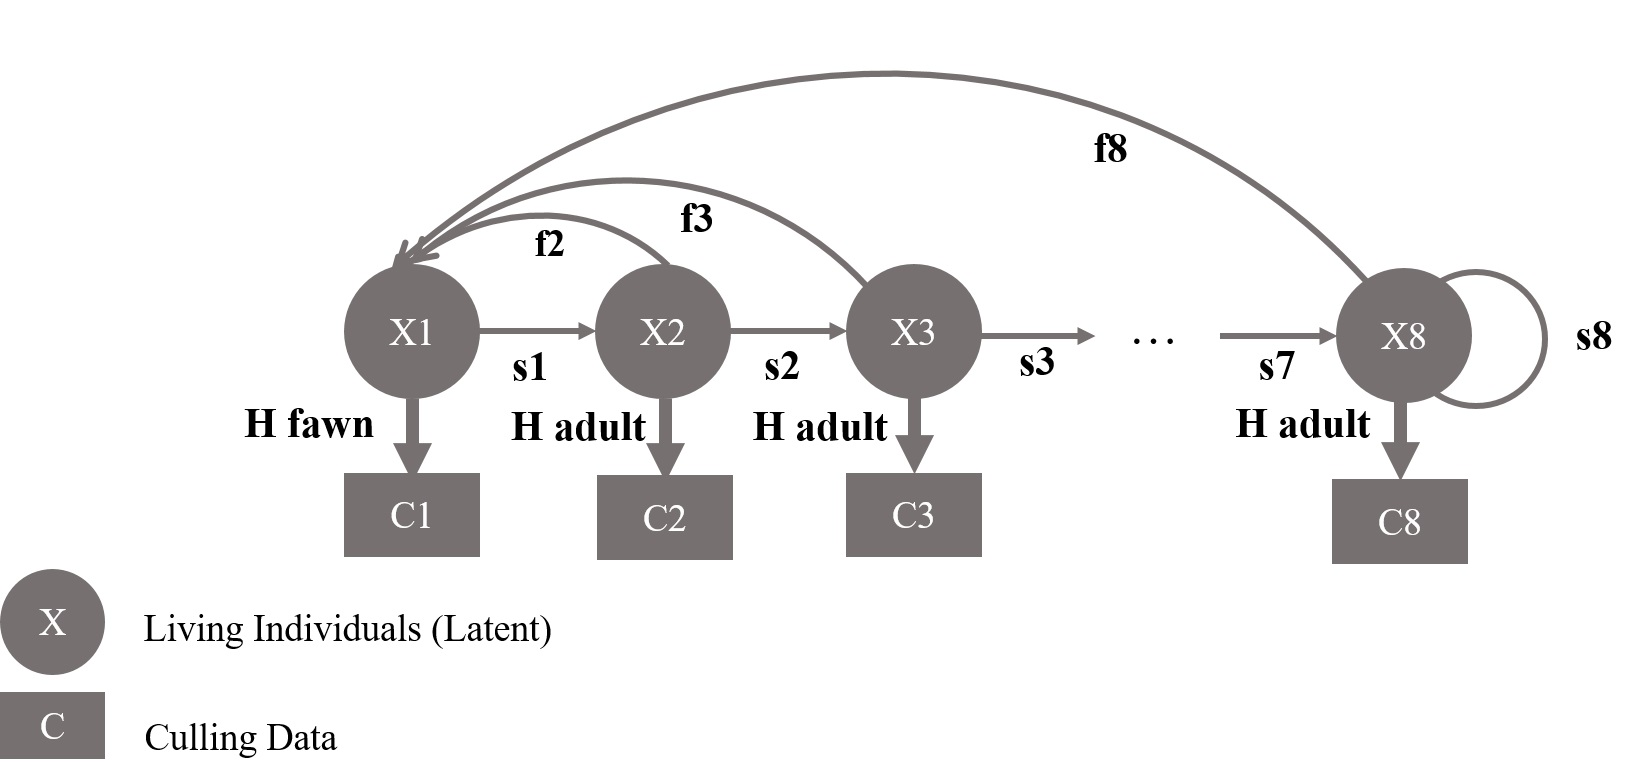
\includegraphics[scale=.18]{fig/Chicago_deer/LHD.jpg}
		%\caption{Wilson}
		\label{LHD}
	\end{figure}
\end{frame}

\subsection{4 Level Bayesian Reconstruction}
\begin{frame}{Bayesian Reconstruction of the Population Dynamics}
	\begin{figure}[ht]
		\centering
		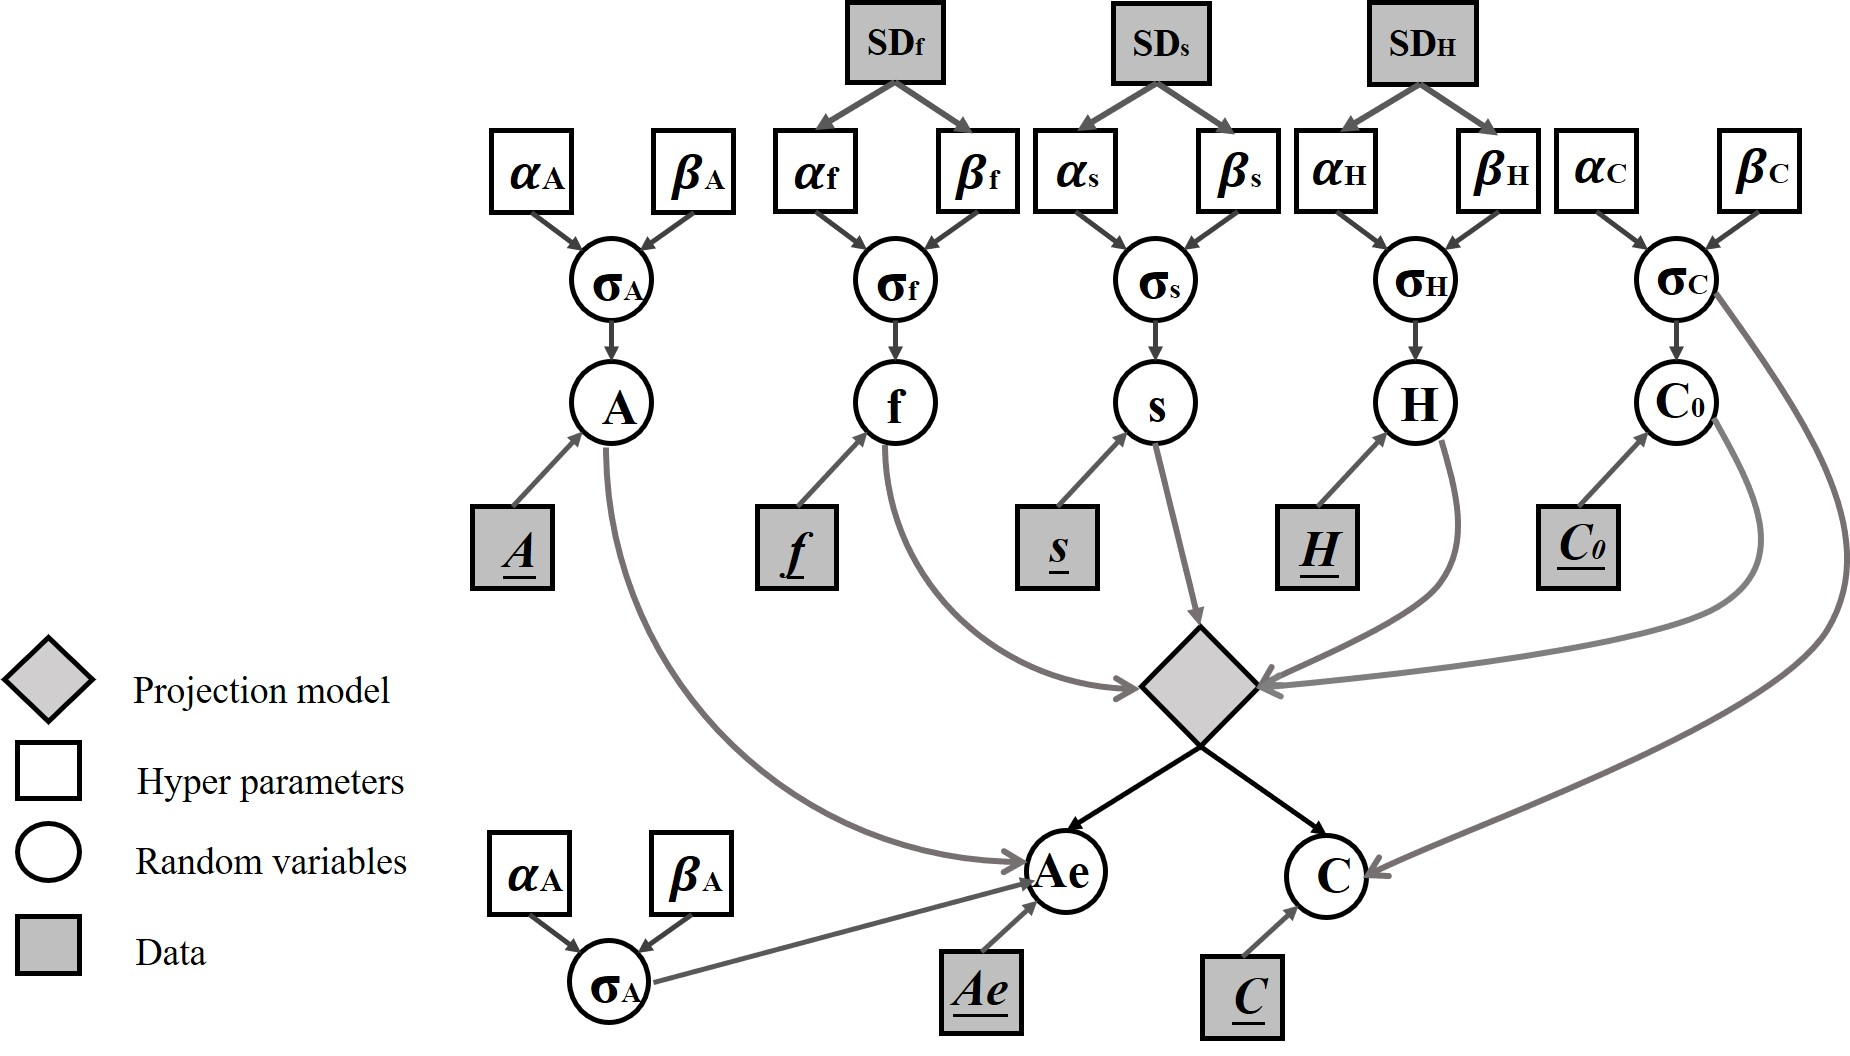
\includegraphics[scale=.25]{fig/Chicago_deer/Bayesian_model_Aerial_count.jpg}
		%\caption{Wilson}
		\label{Bayesian}
	\end{figure}
\end{frame}

\begin{frame}{Bayesian Reconstruction of the Population Dynamics}
	\begin{figure}[ht]
		\centering
		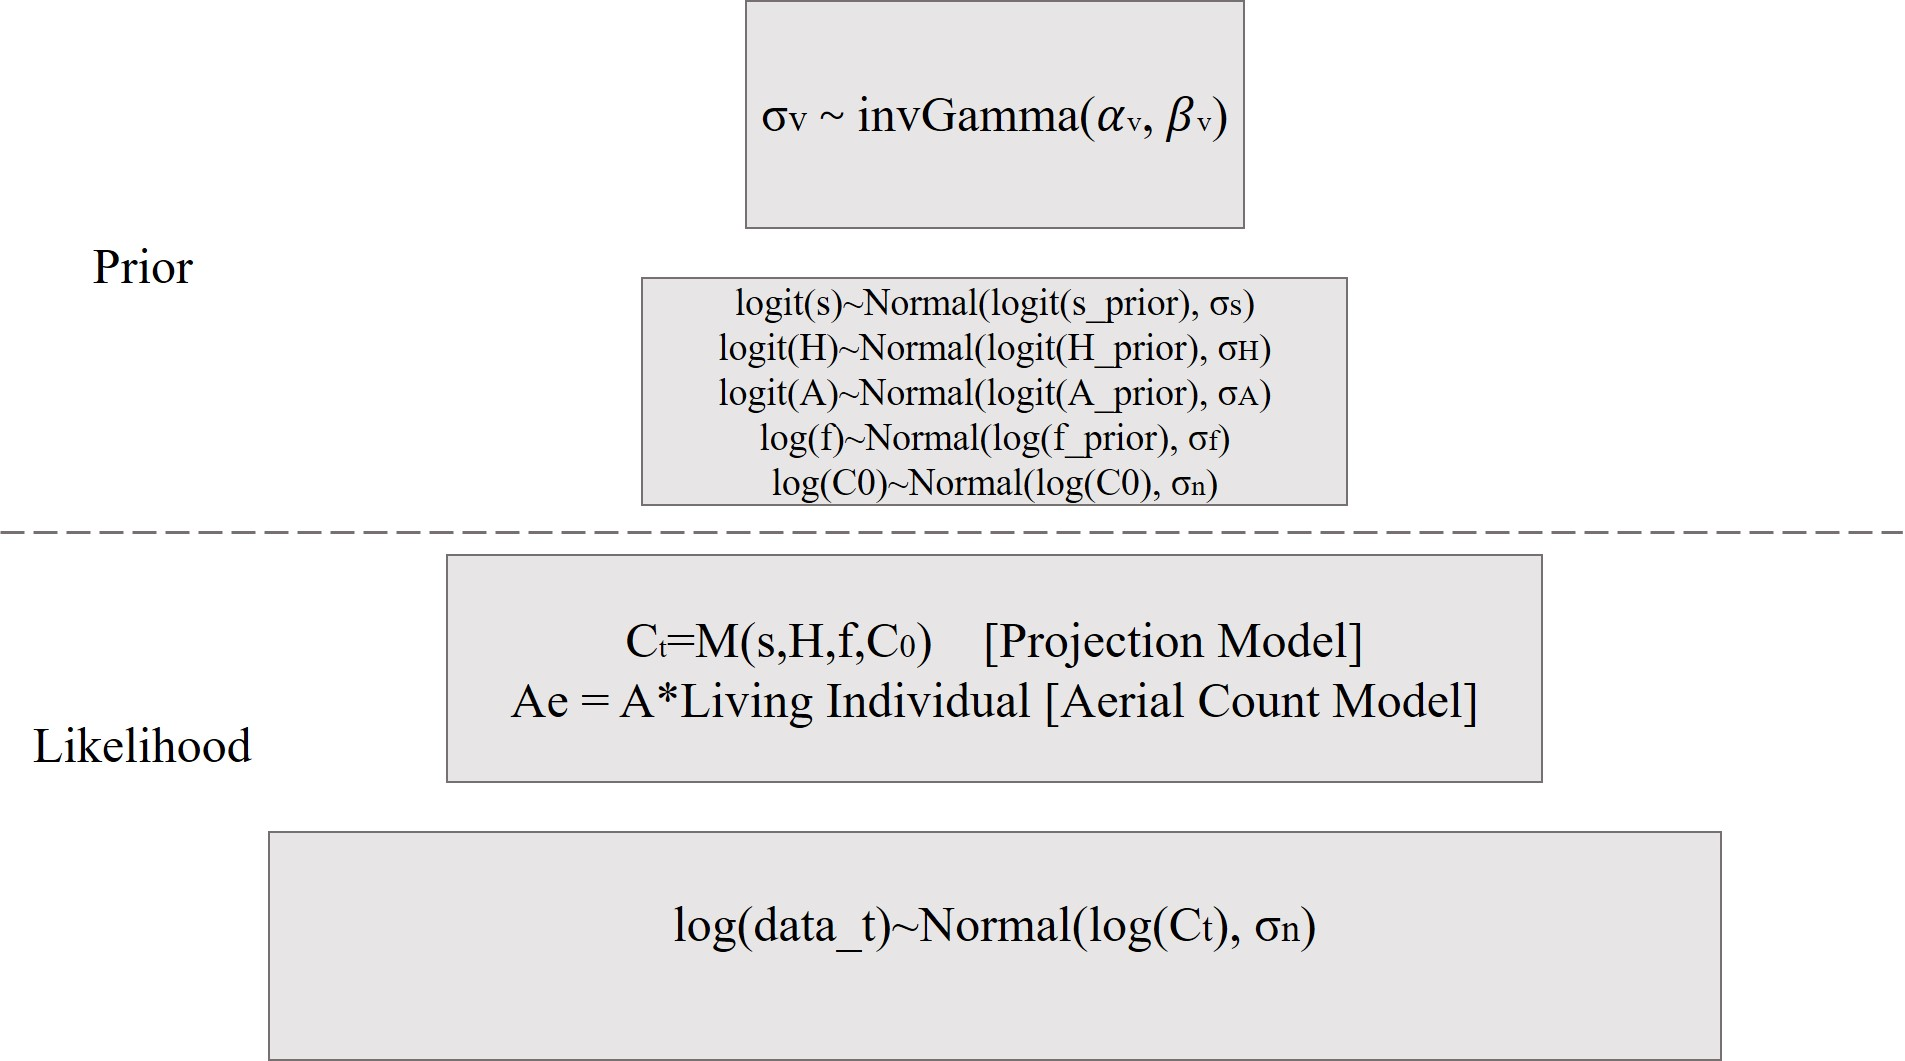
\includegraphics[scale=.25]{fig/Chicago_deer/Bayesian_model_4level_aerial.jpg}
		%\caption{Wilson}
		\label{4level}
	\end{figure}
\end{frame}

\section{Results}
\subsection{Model Checking}
\begin{frame}{Model Checking: Culling}
	\begin{table}[htbp] % model checking table
		\centering
		\caption{\label{tab:check}Model Checking Indexes for Reconstruction of Culling Data}
		\begin{tabular}{ccc}
			\toprule
			&Mean&Standard Error\\
			\midrule
			Absolute Difference&7.69 & 0.911\\
			Posterior Standard Deviation & 12.28 & 0.219\\
			Precision & 91\% & -\\
			\bottomrule
		\end{tabular}
	\end{table}

\end{frame}

\begin{frame}{Model Checking: Aerial Counting}
	\begin{table}[htbp] % model checking table
		\centering
		\caption{\label{tab:check2}Model Checking Indexes for Reconstruction of Aerial Counting Data}
		\begin{tabular}{ccc}
			\toprule
			&Mean&Standard Error\\
			\midrule
			Absolute Difference&108.81 & 0.58\\
			Posterior Standard Deviation & 94.26 & 0.96\\
			Precision & 100\% & -\\
			\bottomrule
		\end{tabular}
	\end{table}
	
\end{frame}

\subsection{Post-Cull Population}
\begin{frame}{Post-Cull Population}
	\begin{figure}[ht]
		\centering
		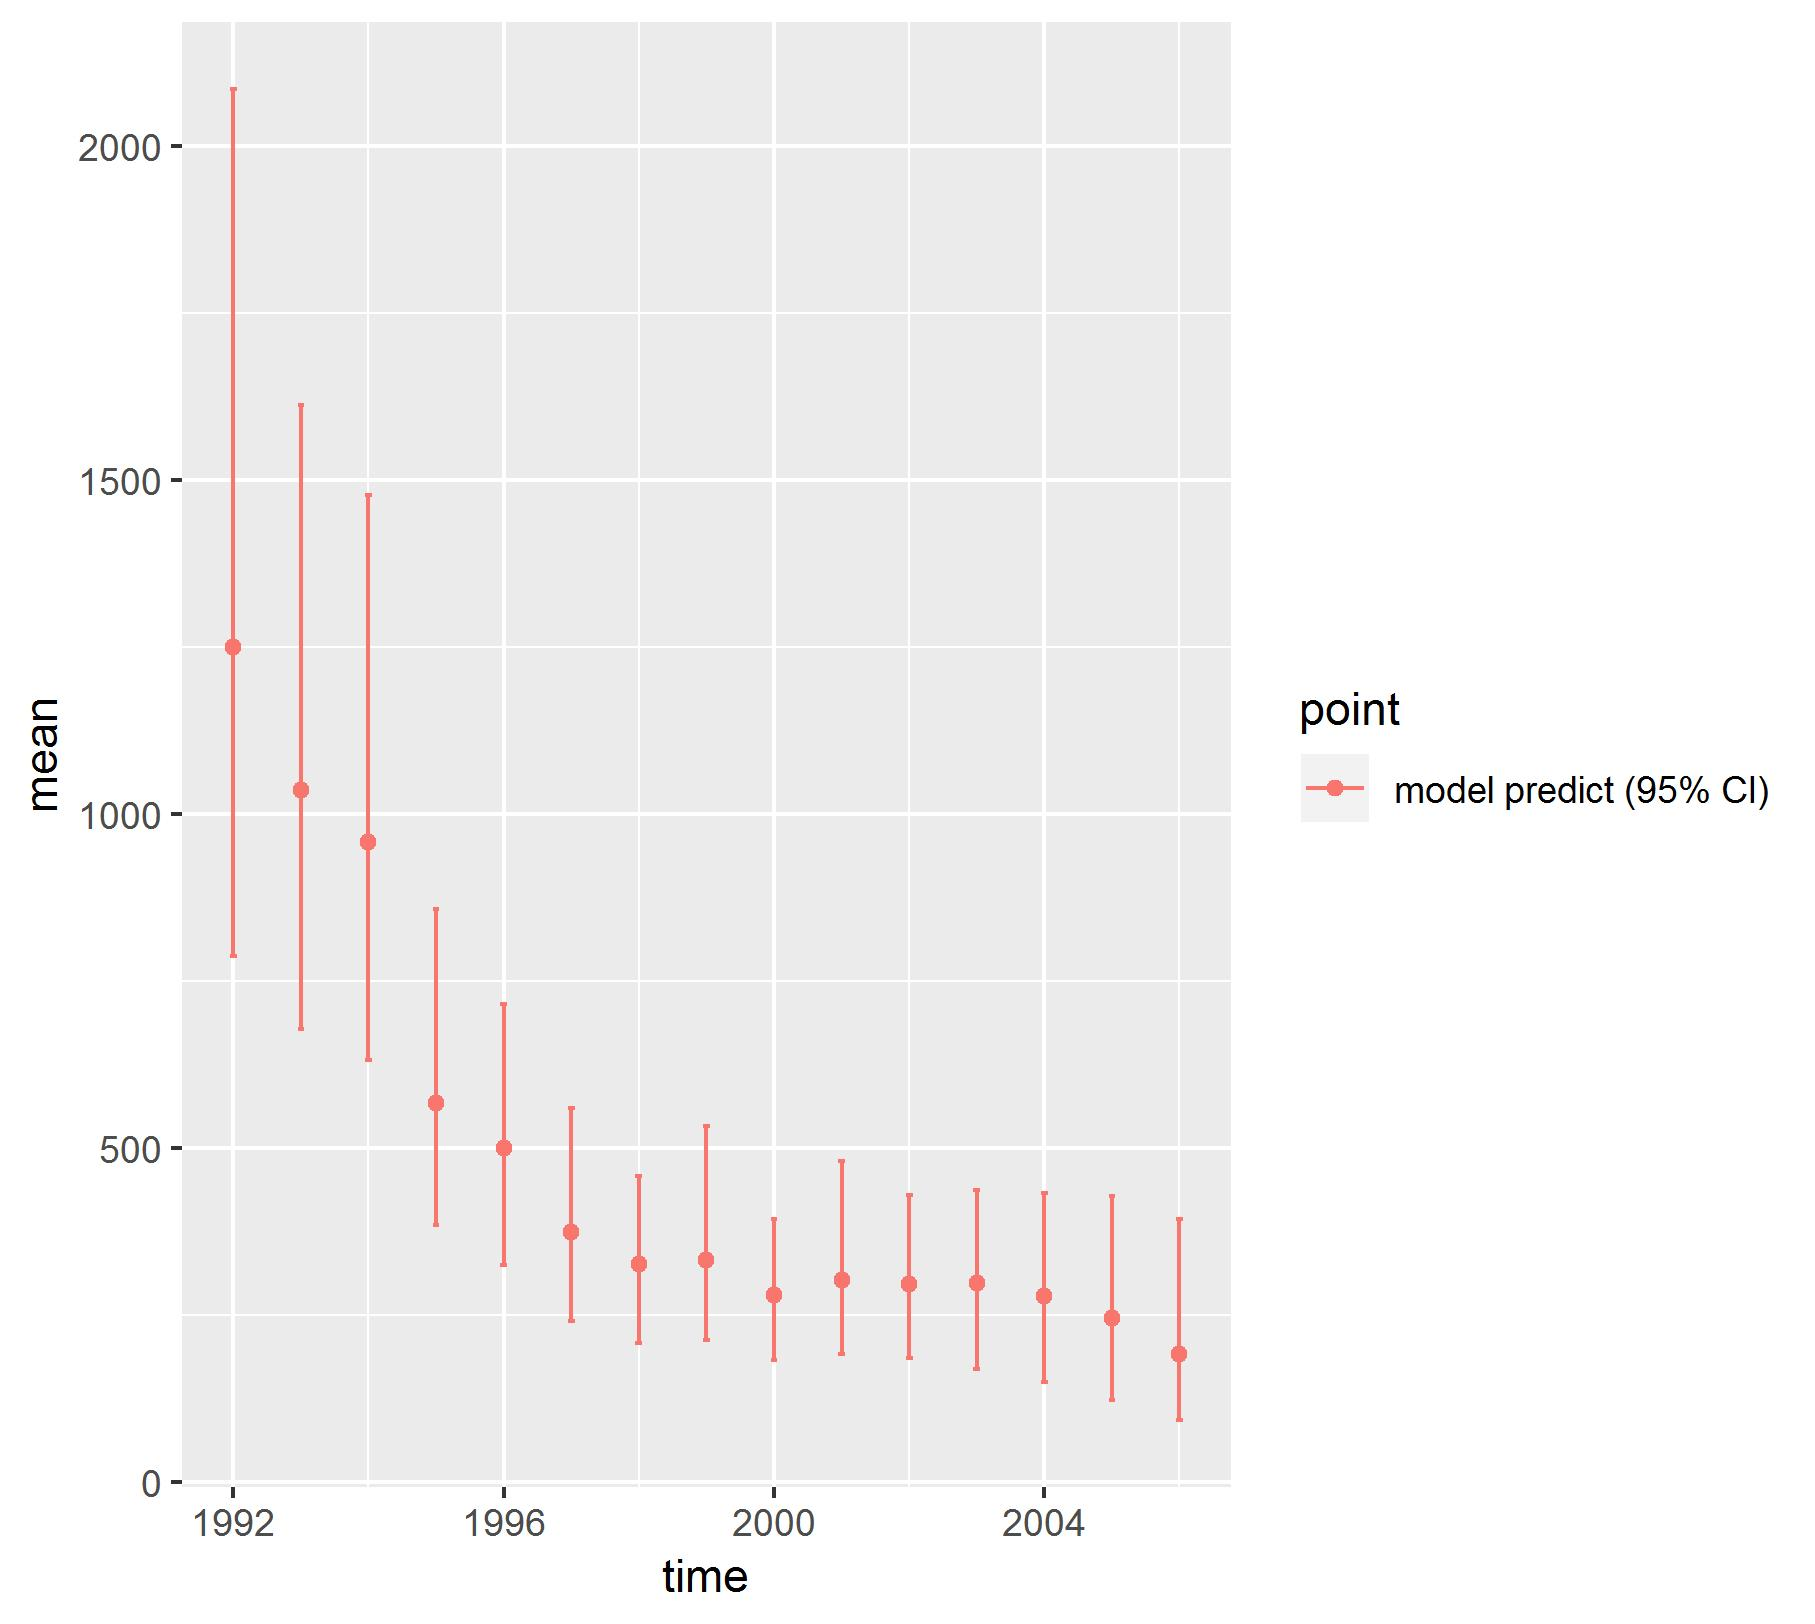
\includegraphics[scale=.45]{fig/Chicago_deer/living_af_culling_all1.jpg}
		%\caption{Wilson}
		\label{postcull}
	\end{figure}
\end{frame}

\subsection{Density Dependency}
\begin{frame}{Density Dependency}
	\begin{itemize}
		\item We detected density dependency on fecundity of most ages
		\item Density dependency on male fawn survival, probability because of dispersion
	\end{itemize}
\end{frame}

\begin{frame}{Density Dependency on Fecundity of Yearlings}
	\begin{figure}[ht]
		\centering
		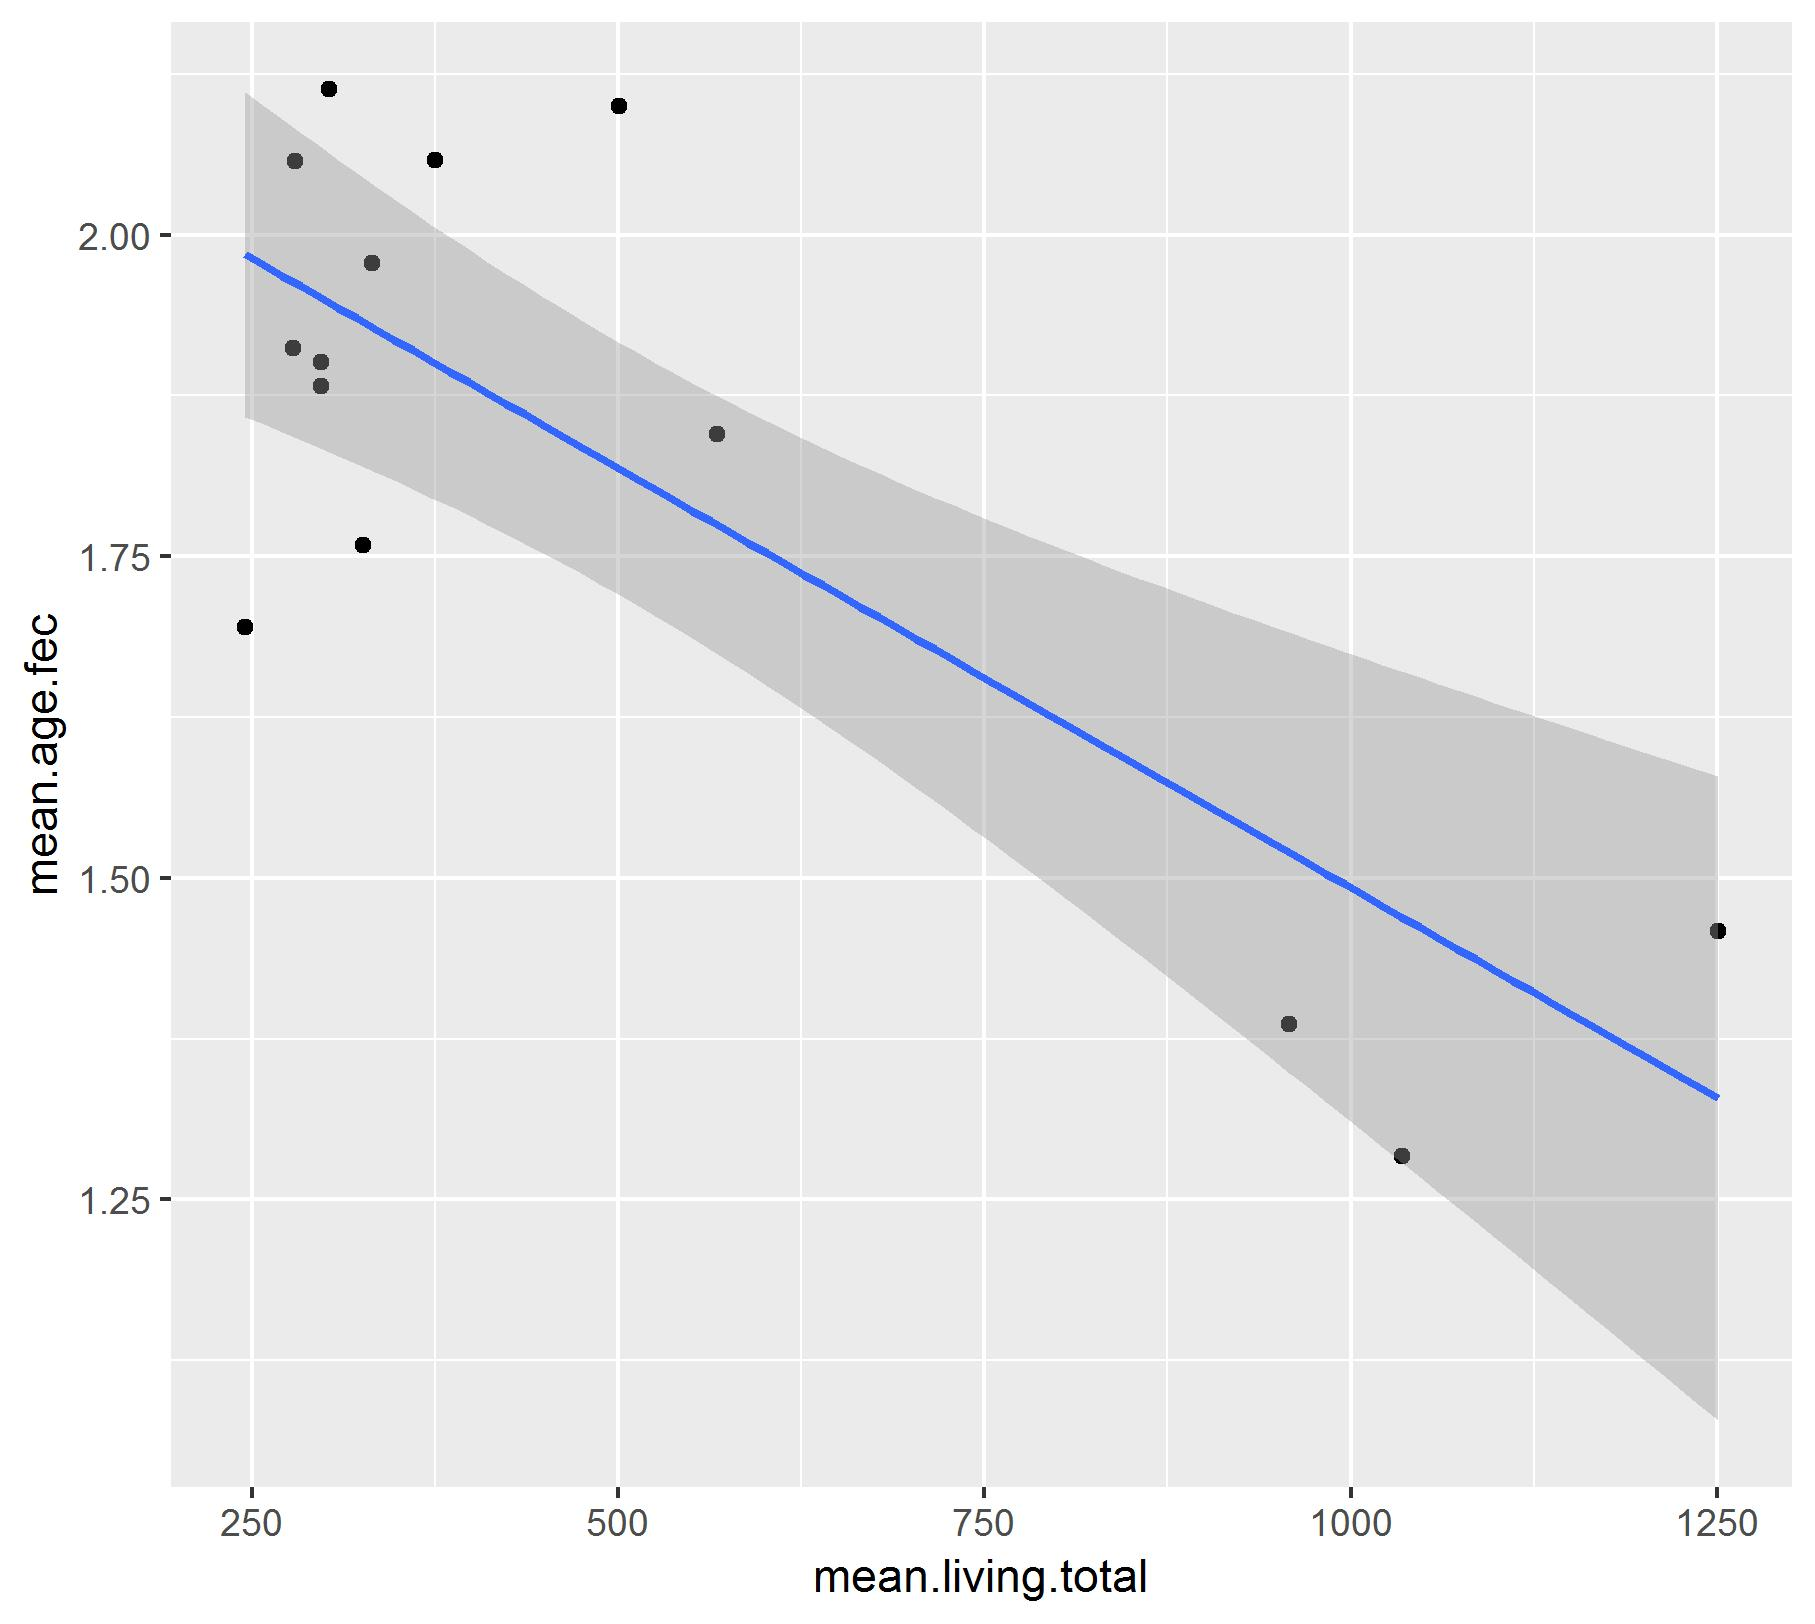
\includegraphics[scale=.45]{fig/Chicago_deer/DDfec_age1.jpg}
		%\caption{Wilson}
		\label{DDfec}
	\end{figure}
\end{frame}

\begin{frame}{Density Dependency on Survival of Male Fawn}
	\begin{figure}[ht]
		\centering
		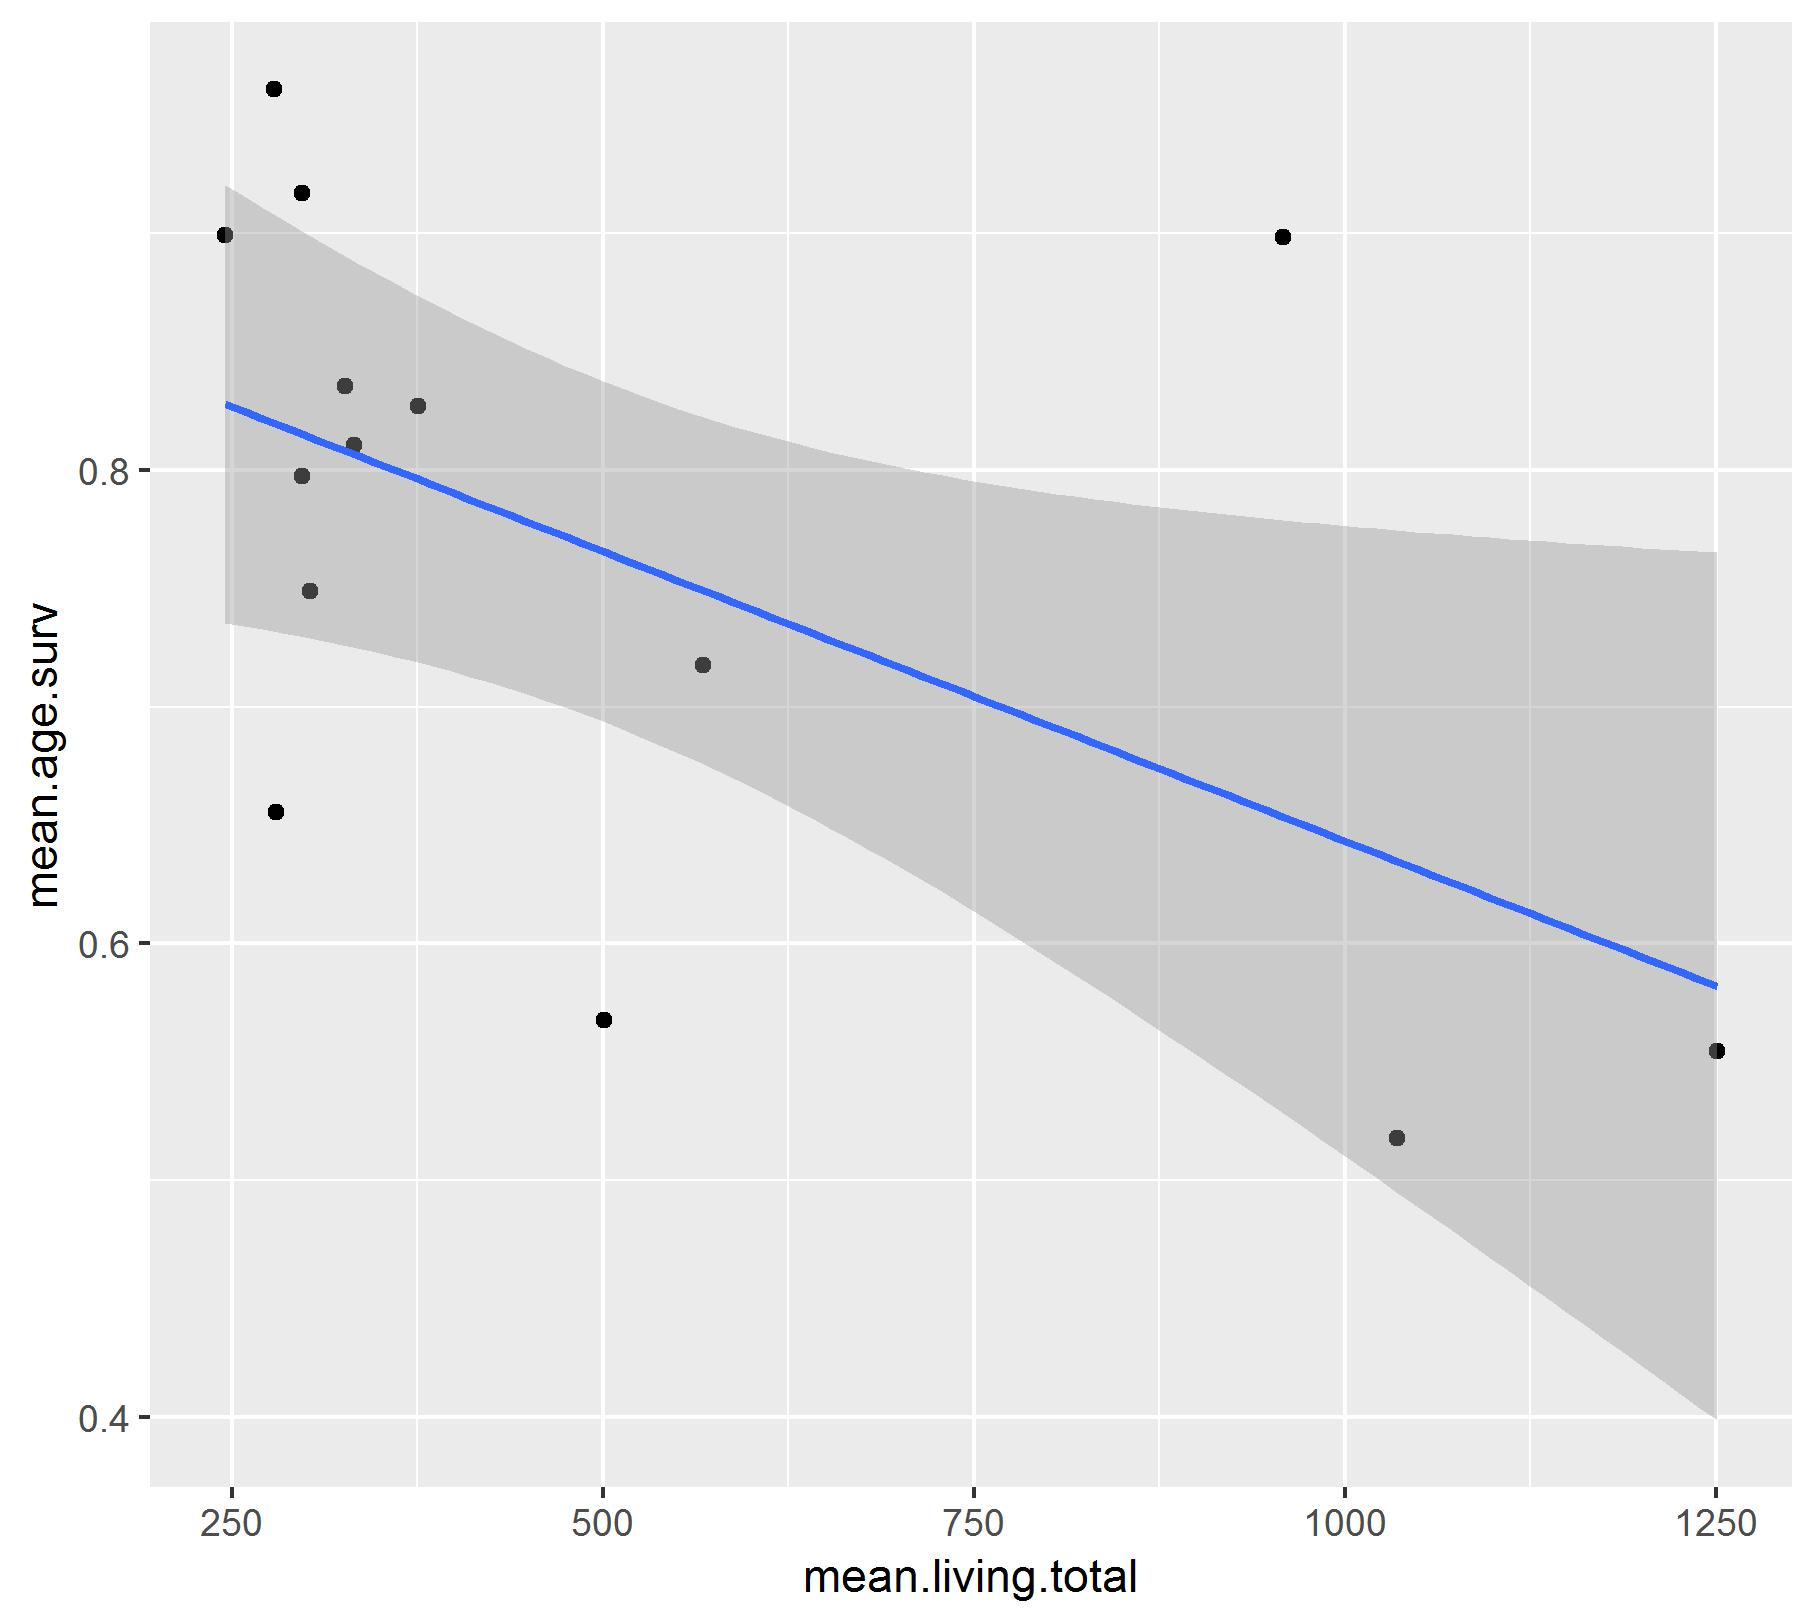
\includegraphics[scale=.45]{fig/Chicago_deer/DDsurv_age9.jpg}
		%\caption{Wilson}
		\label{DDsurv}
	\end{figure}
\end{frame}


\section{Discussion}
\begin{frame}{Density Dependency on Survival of Male Fawn}
	\begin{itemize}
		\item Survival of male fawn is lower than female
		\item White tailed deer is male dispersing.
	\end{itemize}
\end{frame}

\begin{frame}{Further Question from Manager}
	\begin{itemize}
		\item What if we skip a year?
		\item Does density dependency means difficulty in half K?
	\end{itemize}
	
\end{frame}

\begin{frame}
	\huge{Questions and Comments are Welcomed!}
\end{frame}

\begin{frame}
	\Huge{Thank you}
\end{frame}

\end{document}